\documentclass[11pt]{beamer}
\usetheme{Pittsburgh}
\usepackage[utf8]{inputenc}
\usepackage[english]{babel}
\usepackage{amsmath}
\usepackage{amsfonts}
\usepackage{amssymb}
\usepackage{graphicx}
\usepackage{minted}
\author{Anselm Jonas Scholl}
\title{List Fusion}
%\setbeamercovered{transparent}
%\setbeamertemplate{navigation symbols}{}
%\logo{}
\institute{Hamburg Haskell Meetup}
%\date{}
%\subject{}
\begin{document}

\begin{frame}
\titlepage
\end{frame}

\begin{frame}
\tableofcontents
\end{frame}

\section{Motivation}

\begin{frame}[fragile]{Motivation}
	\begin{itemize}
		\item Operations on lists are convenient.
		\item Lots of syntactic sugar, standard library support, ability to stream large data sets, \dots
		\item And lots of allocation!
	\end{itemize}
\end{frame}

\begin{frame}[fragile]{Motivation}
\begin{minted}{haskell}
sqr x = x * x

sumSquares = sum . map sqr

numbers from to = take (to - from + 1)
    $ iterate (+1) from

sumSquaresOfNumbers from to = sumSquares
    $ numbers from to

sumSquaresOfNumbers' from to = go 0 from
  where go !acc n
    | n <= to   = go (acc + sqr n) (n + 1)
    | otherwise = acc
\end{minted}
\end{frame}

\begin{frame}[fragile]{Motivation}
\begin{minted}{haskell}
sqrRem to x = sqr x `rem` to

maximumSqrRem remBy = maximum . map (sqrRem remBy)

numbers from to = take from
    $ enumFromTo 0 to

maximumSqrRemNumbers from to = maximumSqrRem to
    $ numbers from to

maximumSqrRemNumbers' from !to = go (-1) 0
  where go !acc n
    | n < from  = go (max acc (sqrRem to n)) (n + 1)
    | otherwise = acc
\end{minted}

\end{frame}

\begin{frame}[fragile]{Motivation}
\begin{minted}{haskell}
avgHelper (!acc, !len) x = (acc + x, len + 1)

average = uncurry quot . foldl avgHelper (0, 0)

numbers a b count = replicate count a ++ replicate count b

averageOfNumbers a b count = average
    $ numbers a b count

averageOfNumbers' a b count = go1 count 0 0
  where
    go1 0 !acc !len = go2 count acc len
    go1 n !acc !len = go1 (n - 1) (acc + a) (len + 1)
    go2 0 !acc !len = acc `quot` len
    go2 n !acc !len = go2 (n - 1) (acc + b) (len + 1)
\end{minted}
\end{frame}

\begin{frame}{Motivation}
	\begin{figure}
		\centering
		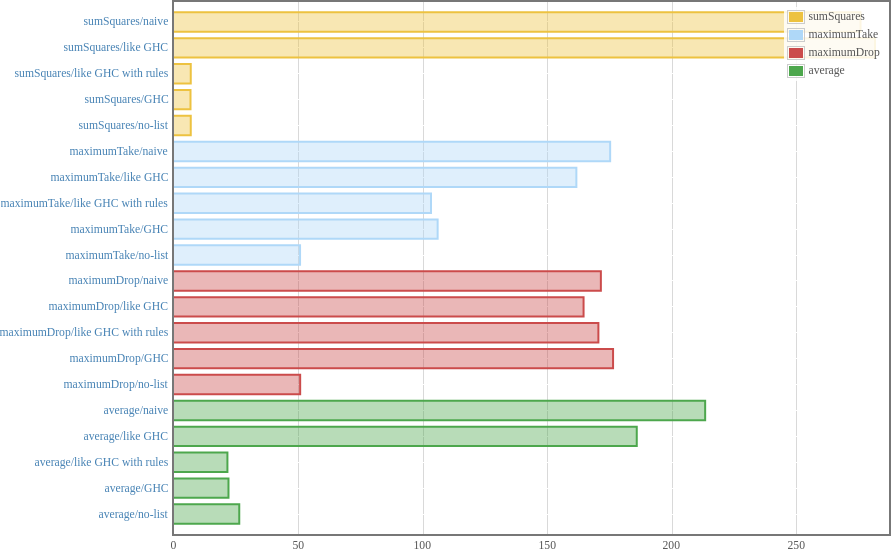
\includegraphics[width=1\textwidth]{benchmark.png}
		\caption{Performance of custom and GHC list functions}
		\label{fig-benchmark}
	\end{figure}
\end{frame}

\begin{frame}{Motivation}
	\begin{itemize}
		\item GHC list functions can get optimized to tight loops.
		\item Even if we copy the implementation of them we still get a lot of allocation.
		\item Only by also copying the rewrite rules used by GHC we achieve a similar runtime.
		\item We can also write specialized functions with the same performance, but they do not compose.
	\end{itemize}
\end{frame}

\section{List Fusion}

\begin{frame}[fragile]{List fusion}
	\begin{itemize}
		\item Two fundamental functions:
			\begin{itemize}
				\item \begin{minted}{haskell}
build :: (forall b. (a -> b -> b) -> b -> b) -> [a]
build g = g (:) []
\end{minted}
				\item \begin{minted}{haskell}
foldr :: (a -> b -> b) -> b -> [a] -> b
foldr k z = go
  where
    go []     = z
    go (y:ys) = y `k` go ys
\end{minted}
			\end{itemize}
		\item If we see \mintinline{C}{foldr k z (build g)}, we replace it with \mintinline{C}{g k z}
		\item[$\rightarrow$] Avoids constructing the list in the first place
		\item[$\rightarrow$] Gives GHC the ability to unbox the list elements
		\item[$\rightarrow$] If done right this gives us a C-like loop
	\end{itemize}
\end{frame}

\subsection{Playing by the Rules}

\begin{frame}[fragile]{Playing by the Rules}
	\begin{itemize}
		\item Instead of hard-coding this rule in the compiler,
			  GHC gives library authors the ability to extend it with
			  additional rewriting rules.
		\item It searches for terms matching the LHS of a rule and
			  replaces then with the RHS of the rule.
		\item GHC does not check that LHS and RHS have the same meaning!
		\item But it makes sure both have the same type.
	\end{itemize}
\end{frame}

\begin{frame}[fragile]{Rules and inlining}
	\begin{itemize}
		\item Rules can only fire on the functions mentioned in a rule.
		\item If a function inlines too early, the rule won't fire.
		\item If a function inlines too late, the rule will not see the correct function and also not fire.
		\item One has to carefully control inlining:
		\begin{itemize}
			\item Inlining happens in phases: 2, 1 and 0.
			\item Each phase the simplifier runs at least once and applies inlining and rewrite rules.
			\item A function can be inlined/not inlined before or starting from a phase.
			\item A rule can also be active before or starting from a phase.
		\end{itemize}
	\end{itemize}
\end{frame}

\begin{frame}[fragile]{Rules and inlining - Example}
\begin{minted}{haskell}
{-# NOINLINE[~1] foo #-}
foo = let x = x in x `seq` ()

{-# RULES "foo terminates" [~1] foo = () #-}

{-# INLINE[1] bar #-}
bar = foo

\end{minted}
\begin{itemize}
	\item We make sure that \mintinline{C}{foo} does not inline while the rule is active.
	\item But \mintinline{C}{bar} is only allowed to inline starting from phase 1.
	\item[$\rightarrow$] \mintinline{C}{bar} will diverge while \mintinline{C}{foo} can be rewritten to \mintinline{C}{()}.
\end{itemize}
\end{frame}

\subsection{Good Producers and Consumers}

\begin{frame}{Good Producers and Consumers}
	\begin{itemize}
		\item A good producer can be fused with a good consumer.
		\item Good producers:
		\begin{itemize}
			\item List comprehensions
			\item Enumerations of Int, Integer, Char
			\item List literals
			\item The cons constructor
			\item (++), map, take, filter, iterate, repeat, zip, zipWith, \dots
		\end{itemize}
		\item Good consumers:
		\begin{itemize}
			\item List comprehensions
			\item array, (++) on the first argument, foldr, map, take, filter, concat, unzip(1,2,3,4), zip, zipWith, partition, head, and, or, any, all, sequence\_, msum, \dots
		\end{itemize}
	\end{itemize}
\end{frame}

\subsection{Fusing map and sum}

\begin{frame}[fragile]{Fusing map and sum}
Let's take a look at the rules for map:
\begin{minted}{haskell}
{-# RULES
"map"       [~1] forall f xs.
  map f xs = build (\c n -> foldr (mapFB c f) n xs)
"mapList"   [1]  forall f.
  foldr (mapFB (:) f) [] = map f
"mapFB"     forall c f g.
  mapFB (mapFB c f) g = mapFB c (f.g)
  #-}
mapFB :: (elt -> lst -> lst)
    -> (a -> elt) -> a -> lst -> lst
{-# INLINE [0] mapFB #-}
mapFB c f = \x ys -> c (f x) ys
\end{minted}
\end{frame}

\begin{frame}[fragile]{Fusing map and sum}
\begin{minted}{haskell}
{-# RULES
"map" [~1] forall f xs.
  map f xs = build (\c n -> foldr (mapFB c f) n xs)
  #-}
\end{minted}
\begin{itemize}
	\item Declares a new rule named ``map''.
	\item The rule is active before phase 1.
	\item \mintinline{C}{f} and \mintinline{C}{xs} are free variables in the rule.
	\item The rule matches on \mintinline{haskell}{map f xs}.
	\item The rule rewrites this to \mintinline{haskell}{build (\c n -> foldr (mapFB c f) n xs)}.
\end{itemize}
\end{frame}

%sum (map f xs)
% > rewrite map
%sum (build (\c n -> foldr (mapFB c f) n xs))
% > inline mapFB
%sum (build (\c n -> foldr (\x ys -> c (f x) ys) n xs))
% > inline sum
%foldl (+) 0 (build (\c n -> foldr (\x ys -> c (f x) ys) n xs))
% > inline foldl
%foldr (\ v fn -> oneShot (\ z -> fn (z + v))) id) (build (\c n -> foldr (\x ys -> c (f x) ys) n xs)) 0
% > fuse foldr and build
%(\c n -> foldr (\x ys -> c (f x) ys) n xs) (\ v fn -> oneShot (\ z -> fn (z + v))) id) 0
% > apply function
%foldr (\x ys -> (\ v fn -> oneShot (\ z -> fn (z + v))) id) (f x) ys) 0 xs
% > apply function
%foldr (\x ys -> oneShot (\ z -> ys (z + f x))) id) 0 xs
%
%foldr (\x ys -> oneShot (\ z -> ys (z + f x))) id) 0 xs



\section{Outlook: Stream Fusion}

\begin{frame}[fragile]{Outlook: Stream Fusion}
	\begin{itemize}
		\item The vector and text libraries use another fusion method: stream fusion
		\item Operations are written as \mintinline{C}{unstream . streamOp . stream}.
		\item Each pair of stream and unstream is removed.
		\item[$\rightarrow$] \mintinline{C}{unstream . opC . stream . unstream . opB . }
			\mintinline{C}{stream . unstream . opA . stream}
		\item[$\rightarrow$] \mintinline{C}{unstream . opC . opB . opA . stream}
	\end{itemize}
\end{frame}

\begin{frame}[fragile]{Outlook: Stream Fusion}
\begin{minted}{haskell}

data Step s a = Done | Skip !s | Yield !a !s

data Stream a = forall s. Stream
  (s -> Step s a) -- stepper function
  !s              -- current state
  !Size           -- size hint

stream :: Text -> Stream Char
unstream :: Stream Char -> Text
\end{minted}
\end{frame}

\begin{frame}[fragile]{Outlook: Stream Fusion}
\begin{minted}{haskell}
data Step s a = Done | Skip s | Yield a s

data Stream m a = forall s. Stream (s -> m (Step s a)) s

data Chunk v a = Chunk Int
  (forall m. (PrimMonad m, Vector v a)
  => Mutable v (PrimState m) a -> m ())

data Bundle m v a = Bundle
  { sElems  :: Stream m a
  , sChunks :: Stream m (Chunk v a)
  , sVector :: Maybe (v a)
  , sSize   :: Size
  }
\end{minted}
\end{frame}

\end{document}
